\documentclass[12pt,a4paper]{article}
\usepackage[utf8]{inputenc}
\usepackage[spanish]{babel}
\usepackage{graphicx}
\usepackage{geometry}
\usepackage{listings}
\usepackage{color}
\usepackage{hyperref}
\usepackage{float}
\usepackage{longtable}
\usepackage{amsmath}

\geometry{top=2.5cm, bottom=2.5cm, left=3cm, right=3cm}

% Configuración
\definecolor{codegreen}{rgb}{0,0.6,0}
\definecolor{codegray}{rgb}{0.5,0.5,0.5}
\definecolor{codepurple}{rgb}{0.58,0,0.82}
\definecolor{backcolour}{rgb}{0.95,0.95,0.92}

\lstdefinestyle{mystyle}{
    backgroundcolor=\color{backcolour},   
    commentstyle=\color{codegreen},
    keywordstyle=\color{magenta},
    numberstyle=\tiny\color{codegray},
    stringstyle=\color{codepurple},
    basicstyle=\ttfamily\footnotesize,
    breakatwhitespace=false,         
    breaklines=true,                 
    captionpos=b,                    
    keepspaces=true,                 
    numbers=left,                    
    numbersep=5pt,                  
    showspaces=false,                
    showstringspaces=false,
    showtabs=false,                  
    tabsize=2,
    language=SQL
}
\lstset{style=mystyle}

\title{Reporte Técnico: PetConnect}
\author{Integrantes del Equipo: \\ Sayuri Herrera Moreno \\ Jiménez Balderas Evelyn Monserrat }
\date{\today}

\begin{document}

% 1. Portada
\begin{titlepage}
    \centering
    {\scshape\LARGE Instituto Politécnico Nacional \par}
    {\scshape\Large Escuela Superior de Cómputo \par}
    \vspace{1cm}
    {\scshape\Large Bases de Datos \par}
    \vspace{1.5cm}
    {\huge\bfseries DataSphere Consultoría: PetConnect \par}
    \vspace{2cm}
    {\Large\itshape Integrantes: \par}
    Sayuri Herrera Moreno \\
    Jiménez Balderas Evelyn Monserrat \\
    \vfill
    Profesor: Ulises Velez Saldaña \\
    Grupo: 3AM1
    \vfill
    {\large \today \par}
\end{titlepage}

% 2. Índices
\tableofcontents
\newpage
% \listoftables
% \newpage
\listoffigures
\newpage

% 3. Definición del Proyecto
\section{Definición del Proyecto}
\subsection{Datos de la Consultora}
\begin{itemize}
    \item \textbf{Nombre de la empresa}: DataSphere Consultoría.
    \item \textbf{Misión}: Brindar soluciones innovadoras a las empresas con proyección ética de impacto social.
    \item \textbf{Visión}: Convertirnos en la consultora internacional de referencia en datos éticos, impulsando innovación y confianza en organizaciones responsables.
    \item \textbf{Nombre del proyecto}: PetConnect.
\end{itemize}

\subsection{Objetivo del Proyecto}
Desarrollar e implementar una plataforma web centralizada que optimice el proceso de adopción de mascotas para una organización con múltiples albergues en Ciudad de México y un sector del Estado de México mediante el uso de algoritmos de compatibilidad que garanticen la eficiencia administrativa y el bienestar animal.

\subsection{Perfiles de Usuario}
\begin{enumerate}
    \item \textbf{Adoptante}: Usuario final interesado en adoptar una mascota.
    \item \textbf{Fundación (Administrador)}: Organización encargada de rescatar y dar en adopción a las mascotas.
\end{enumerate}

\subsection{Funciones por Usuario}
\subsubsection{Adoptante}
\begin{itemize}
    \item Registrarse e iniciar sesión.
    \item Gestionar su perfil personal y datos demográficos (CP, ubicación).
    \item Buscar y filtrar mascotas por especie, tamaño, edad.
    \item Ver detalles completos de la mascota (historial médico, vacunas y padecimientos).
    \item Enviar solicitudes de adopción.
    \item Consultar el estado de sus solicitudes.
    \item Hacer donaciones.
    \item Agendar citas de visita a la fundación.
\end{itemize}
\subsubsection{Fundación}
\begin{itemize}
    \item Registrar nuevas mascotas rescatadas con foto y detalles.
    \item Gestionar el expediente médico (vacunas, padecimientos, eventos).
    \item Visualizar solicitudes de adopción entrantes.
    \item Aprobar o rechazar solicitudes.
    \item Gestionar donaciones recibidas.
    \item Visualizar y agregar dueños en lista negra.
    \item Gestionar rescates de mascotas.
    \item Agregar y añadir colaboradores.
\end{itemize}

\subsection{Información de Principales Entidades}
El sistema almacena información sobre:
\begin{itemize}
    \item \textbf{Mascota Rescatada}: Datos físicos (especie, raza, tamaño, color), comportamiento, fotos, señas particulares.
    \item \textbf{Rescate}: Fecha, alcaldía (municipio), situación del rescate, necesidades especiales.
    \item \textbf{Historial Médico}: 
    \begin{itemize}
        \item \textbf{Eventos Médicos}: Desparasitaciones, cirugías, tratamientos.
        \item \textbf{Vacunas}: Registro de vacunas aplicadas y próximas dosis.
        \item \textbf{Padecimientos}: Enfermedades crónicas y sus tratamientos.
    \end{itemize}
    \item \textbf{Solicitud de Adopción}: Vínculo entre adoptante y mascota con estado (pendiente, aprobada, rechazada).
    \item \textbf{Usuarios (Auth)}: Sistema de autenticación con roles (fundación, adoptante).
    \item \textbf{Empleados y Sucursales}: Estructura organizacional de la fundación, incluyendo historial de asignaciones y asistencias.
    \item \textbf{Adoptante Perfil}: Información detallada del adoptante (tipo de vivienda, experiencia previa, composición del hogar) para determinar idoneidad.
    \item \textbf{Donaciones}: Registro de aportaciones económicas de donadores.
\end{itemize}

\subsection{Arquitectura}
\begin{itemize}
    \item \textbf{Tipo de Aplicación}: Web (Cliente-Servidor).
    \item \textbf{Frontend}: HTML5, CSS3, JavaScript (Vanilla ES6+).
    \item \textbf{Backend}: Python 3.10+ con FastAPI (Framework REST).
    \item \textbf{Base de Datos}: PostgreSQL 14+.
    \item \textbf{Comunicación}: API REST via fetch/HTTP.
\end{itemize}

% 4. Diseño de la Base de Datos
\section{Diseño de la Base de Datos}

\subsection{Entidades Principales}
\begin{itemize}
    \item \textbf{mascota\_rescatada}:
    \begin{itemize}
        \item PK: \texttt{id\_mascota} (INT)
        \item FK: \texttt{id\_raza}, \texttt{id\_origen} (Fundación)
        \item Atriubtos: nombre, edad, sexo, tamaño, comportamiento, url\_foto.
    \end{itemize}
    
    \item \textbf{rescate}:
    \begin{itemize}
        \item PK: \texttt{id\_rescate}
        \item FK: \texttt{id\_mascota} (Relación 1:1)
        \item Atributos: fecha, alcaldía, situación, necesidades\_especiales.
    \end{itemize}

    \item \textbf{solicitud\_adopcion}:
    \begin{itemize}
        \item PK: \texttt{id\_solicitud}
        \item FK: \texttt{id\_adoptante}, \texttt{id\_mascota}
        \item Atributos: fecha\_solicitud, estado, motivo\_rechazo.
    \end{itemize}
    
    \item \textbf{fundacion}:
    \begin{itemize}
        \item PK: \texttt{id\_fundacion} (SERIAL)
        \item Atributos: nombre, email, telefono, rfc.
    \end{itemize}
    
    \item \textbf{adoptante\_perfil}:
    \begin{itemize}
        \item PK: \texttt{id\_adoptante} (FK de adoptante)
        \item Atributos: tipo\_vivienda, tiene\_patio, nivel\_economico, experiencia\_previa.
    \end{itemize}
\end{itemize}

\subsection{Relaciones}
\begin{itemize}
    \item \textbf{Fundación - Mascota}: 1:N (Una fundación registra muchas mascotas).
    \item \textbf{Mascota - Solicitud}: 1:N (Una mascota puede tener varias solicitudes, aunque solo se aprueba una).
    \item \textbf{Adoptante - Solicitud}: 1:N (Un adoptante puede hacer varias solicitudes).
    \item \textbf{Mascota - Vacuna}: N:M (Implementada via \texttt{vacuna\_aplicada}).
    \item \textbf{Empleado - Sucursal}: N:M (Histórico mediante \texttt{empleado\_sucursal\_hist}).
\end{itemize}

\begin{figure}[H]
    \centering
    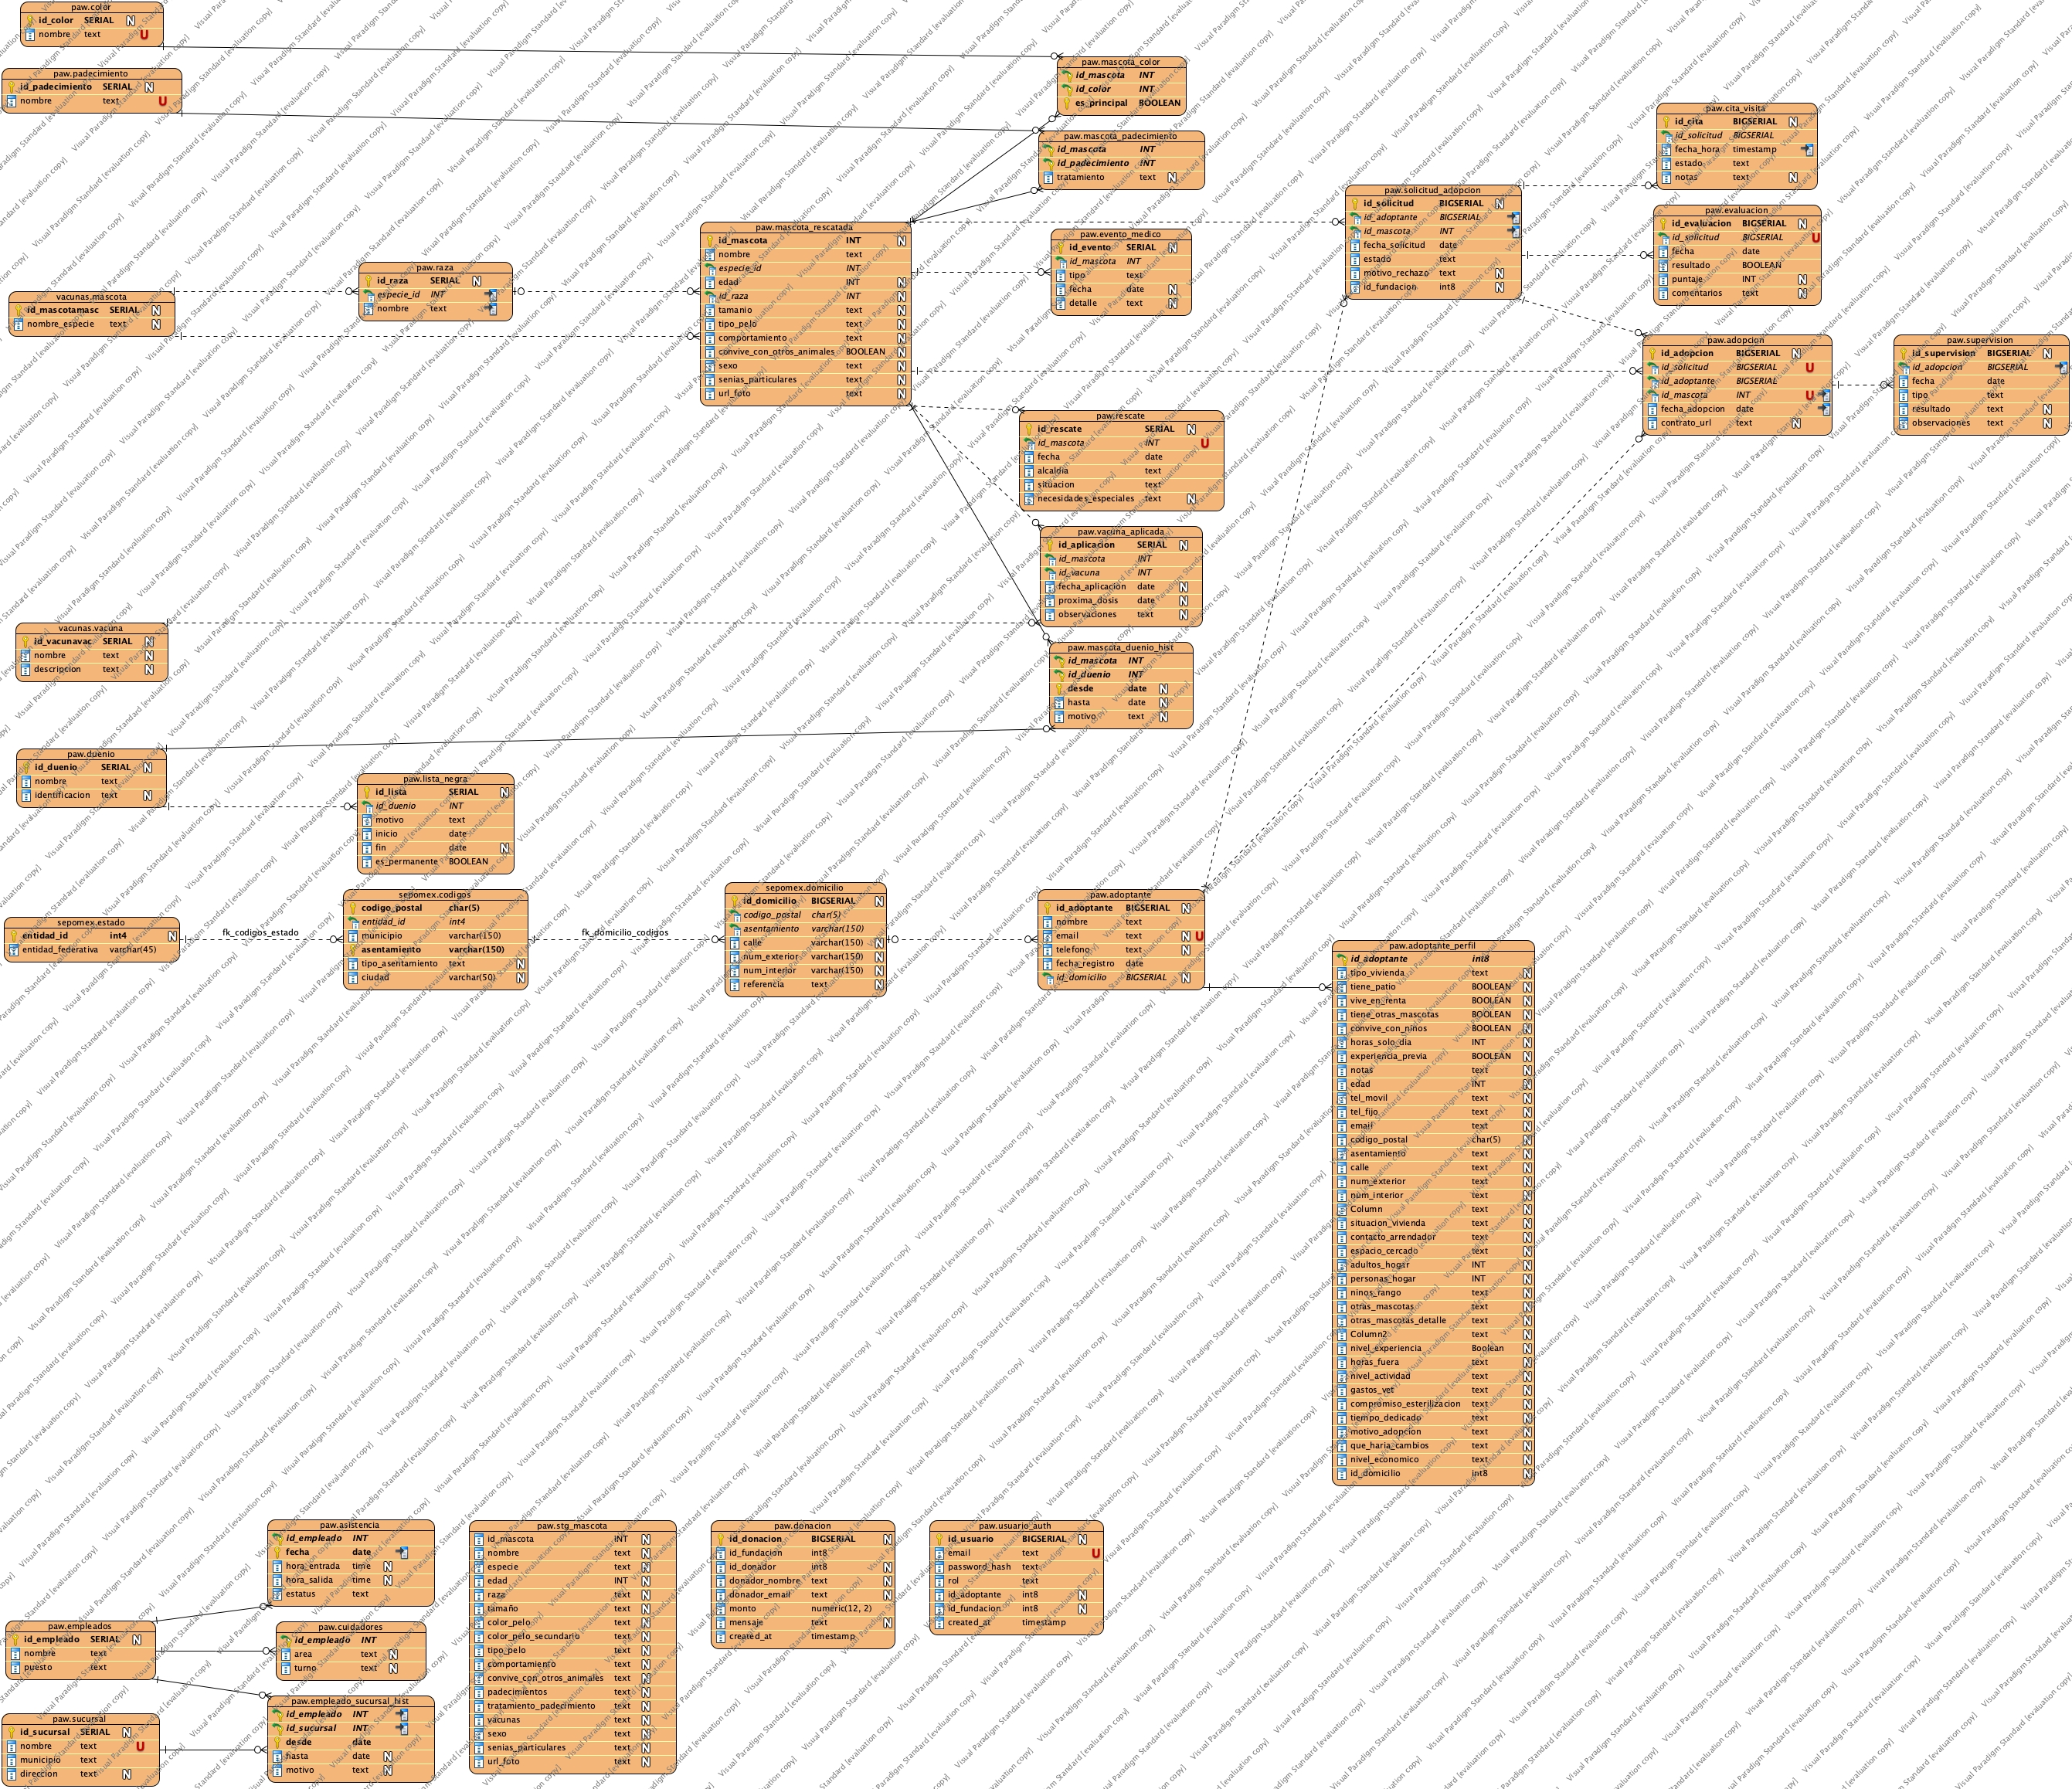
\includegraphics[width=1.0\textwidth]{diagrama_er.jpg}
    \caption{Diagrama Entidad-Relación (Generado en Visual Paradigm)}
    \label{fig:diagrama_er}
\end{figure}

% 5. Diccionario de Datos
\section{Diccionario de Datos}

\begin{longtable}{|p{3.5cm}|p{2cm}|p{1cm}|p{1.5cm}|p{5cm}|}
\hline
\textbf{Campo} & \textbf{Tipo} & \textbf{Nulo} & \textbf{Llave} & \textbf{Descripción} \\
\hline
\multicolumn{5}{|c|}{\textbf{Tabla: mascota\_rescatada}} \\
\hline
id\_mascota & INT & No & PK & Identificador único de la mascota. \\
nombre & TEXT & No & & Nombre de la mascota. \\
edad & INT & Si & & Edad aproximada en años. \\
id\_origen & INT & No & FK & ID de la fundación que la registró. \\
especie\_id & INT & No & FK & Clasificación (1=perro, 2=gato). \\
tamanio & TEXT & Si & & Tamaño (pequeño, mediano, grande). \\
\hline
\multicolumn{5}{|c|}{\textbf{Tabla: rescate}} \\
\hline
id\_rescate & SERIAL & No & PK & Identificador del evento de rescate. \\
id\_mascota & INT & No & FK/U & Vínculo con la mascota (1:1). \\
fecha & DATE & No & & Fecha del rescate. \\
alcaldia & TEXT & No & & Lugar donde fue encontrado. \\
\hline
\multicolumn{5}{|c|}{\textbf{Tabla: solicitud\_adopcion}} \\
\hline
id\_solicitud & BIGSERIAL & No & PK & Folio único de la solicitud. \\
id\_adoptante & BIGINT & No & FK & Usuario que solicita. \\
id\_mascota & INT & No & FK & Mascota solicitada. \\
estado & TEXT & No & & pendiente, aprobada, rechazada. \\
\hline
\end{longtable}

% 6. Diseño de Interfaces
\section{Diseño de Interfaces}

El sistema implementa una arquitectura de Aplicación de Página Única (SPA) donde la navegación es fluida y dinámica sin recargas completas de página. Las interfaces se adaptan automáticamente según el rol del usuario autenticado.

\subsection{Mapa de Navegación}
\begin{enumerate}
    \item \textbf{Módulo de Acceso}:
    \begin{itemize}
        \item Pantalla de Bienvenida (Landing Page con estadísticas).
        \item Login (Validación de credenciales y redirección por rol).
        \item Registro de Adoptante (Creación de cuenta básica).
    \end{itemize}
    
    \item \textbf{Panel del Adoptante}:
    \begin{itemize}
        \item \textbf{Mi Perfil}: Formulario extenso de idoneidad (Datos personales, vivienda, estilo de vida).
        \item \textbf{Buscar Mascotas}: Catálogo con filtros dinámicos (Especie, Edad, Tamaño).
        \item \textbf{Mis Solicitudes}: Seguimiento de estado (Pendiente, Aprobada, Rechazada).
        \item \textbf{Citas de Visita}: Agendamiento de visitas al albergue.
        \item \textbf{Donaciones}: Realizar donaciones.
    \end{itemize}

    \item \textbf{Panel de Fundación}:
    \begin{itemize}
        \item \textbf{Gestión de Mascotas}: Alta de nuevas mascotas y consulta de inventario.
        \item \textbf{Rescates}: Registro detallado de eventos de rescate (Ubicación, Situación).
        \item \textbf{Solicitudes}: Bandeja de entrada para aprobar/rechazar adopciones.
        \item \textbf{Lista Negra}: Gestión de dueños vetados por maltrato.
        \item \textbf{Colaboradores}: Alta de empleados (Veterinarios, Cuidadores).
        \item \textbf{Donaciones}: Visualización de aportaciones recibidas.
    \end{itemize}
\end{enumerate}

\subsection{Detalle de Pantallas Principales}

\subsubsection{1. Catálogo de Adopción (Adoptante)}
Interfaz visual tipo "Grid" que muestra tarjetas de mascotas disponibles.
\begin{itemize}
    \item \textbf{Filtros Laterales}: Permiten refinar la búsqueda por especie (Perro/Gato), edad, tamaño y un filtro especial de "Compatibilidad Sugerida".
    \item \textbf{Interacción}: Al hacer clic en una tarjeta, se abre el modal de detalles.
\end{itemize}

\begin{figure}[H]
    \centering
    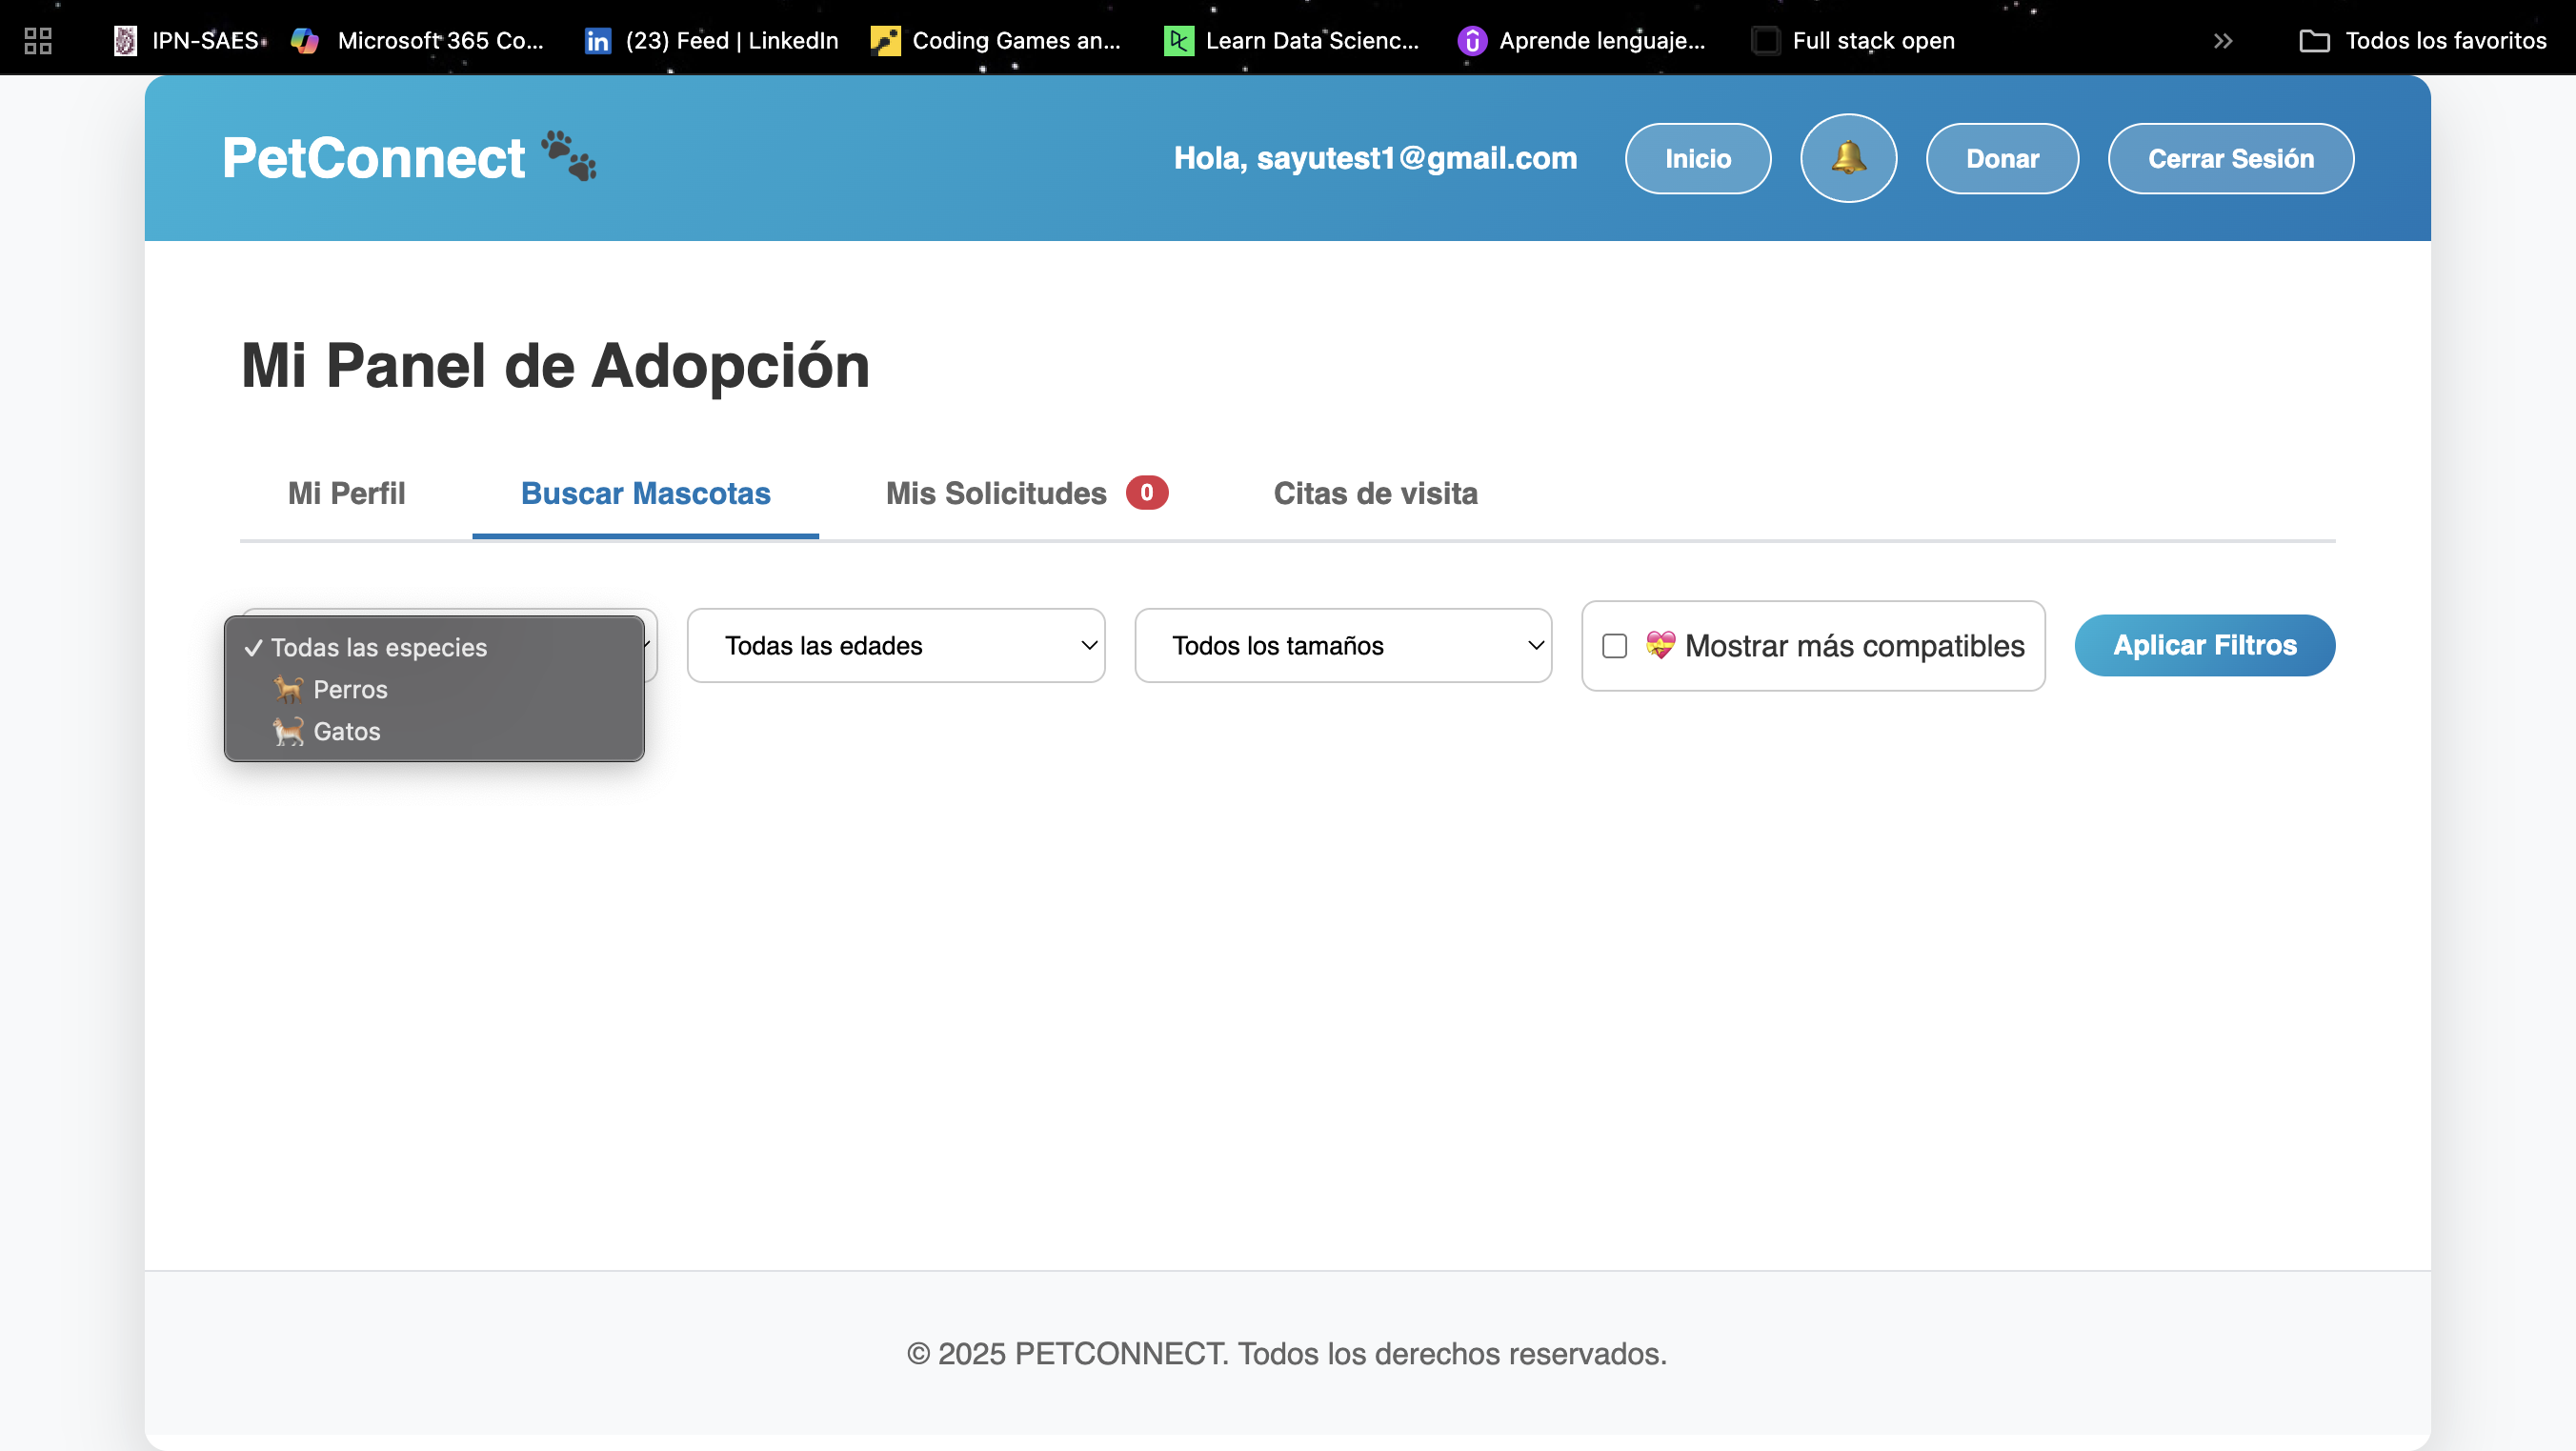
\includegraphics[width=0.8\textwidth]{Filtrado de mascotas.png} 
    \caption{Interfaz del Catálogo de Adopción}
    \label{fig:catalogo}
\end{figure}

\subsubsection{2. Modal de Detalles de Mascota}
Ventana emergente completa que muestra:
\begin{itemize}
    \item Fotografía en alta resolución.
    \item Historia del rescate y necesidades especiales.
    \item \textbf{Datos Clínicos}: Tablas con historial de vacunas, padecimientos y tratamientos.
    \item \textbf{Acción}: Botón "Solicitar Adopción" (bloqueado si el perfil no está completo).
\end{itemize}

\begin{figure}[H]
    \centering
    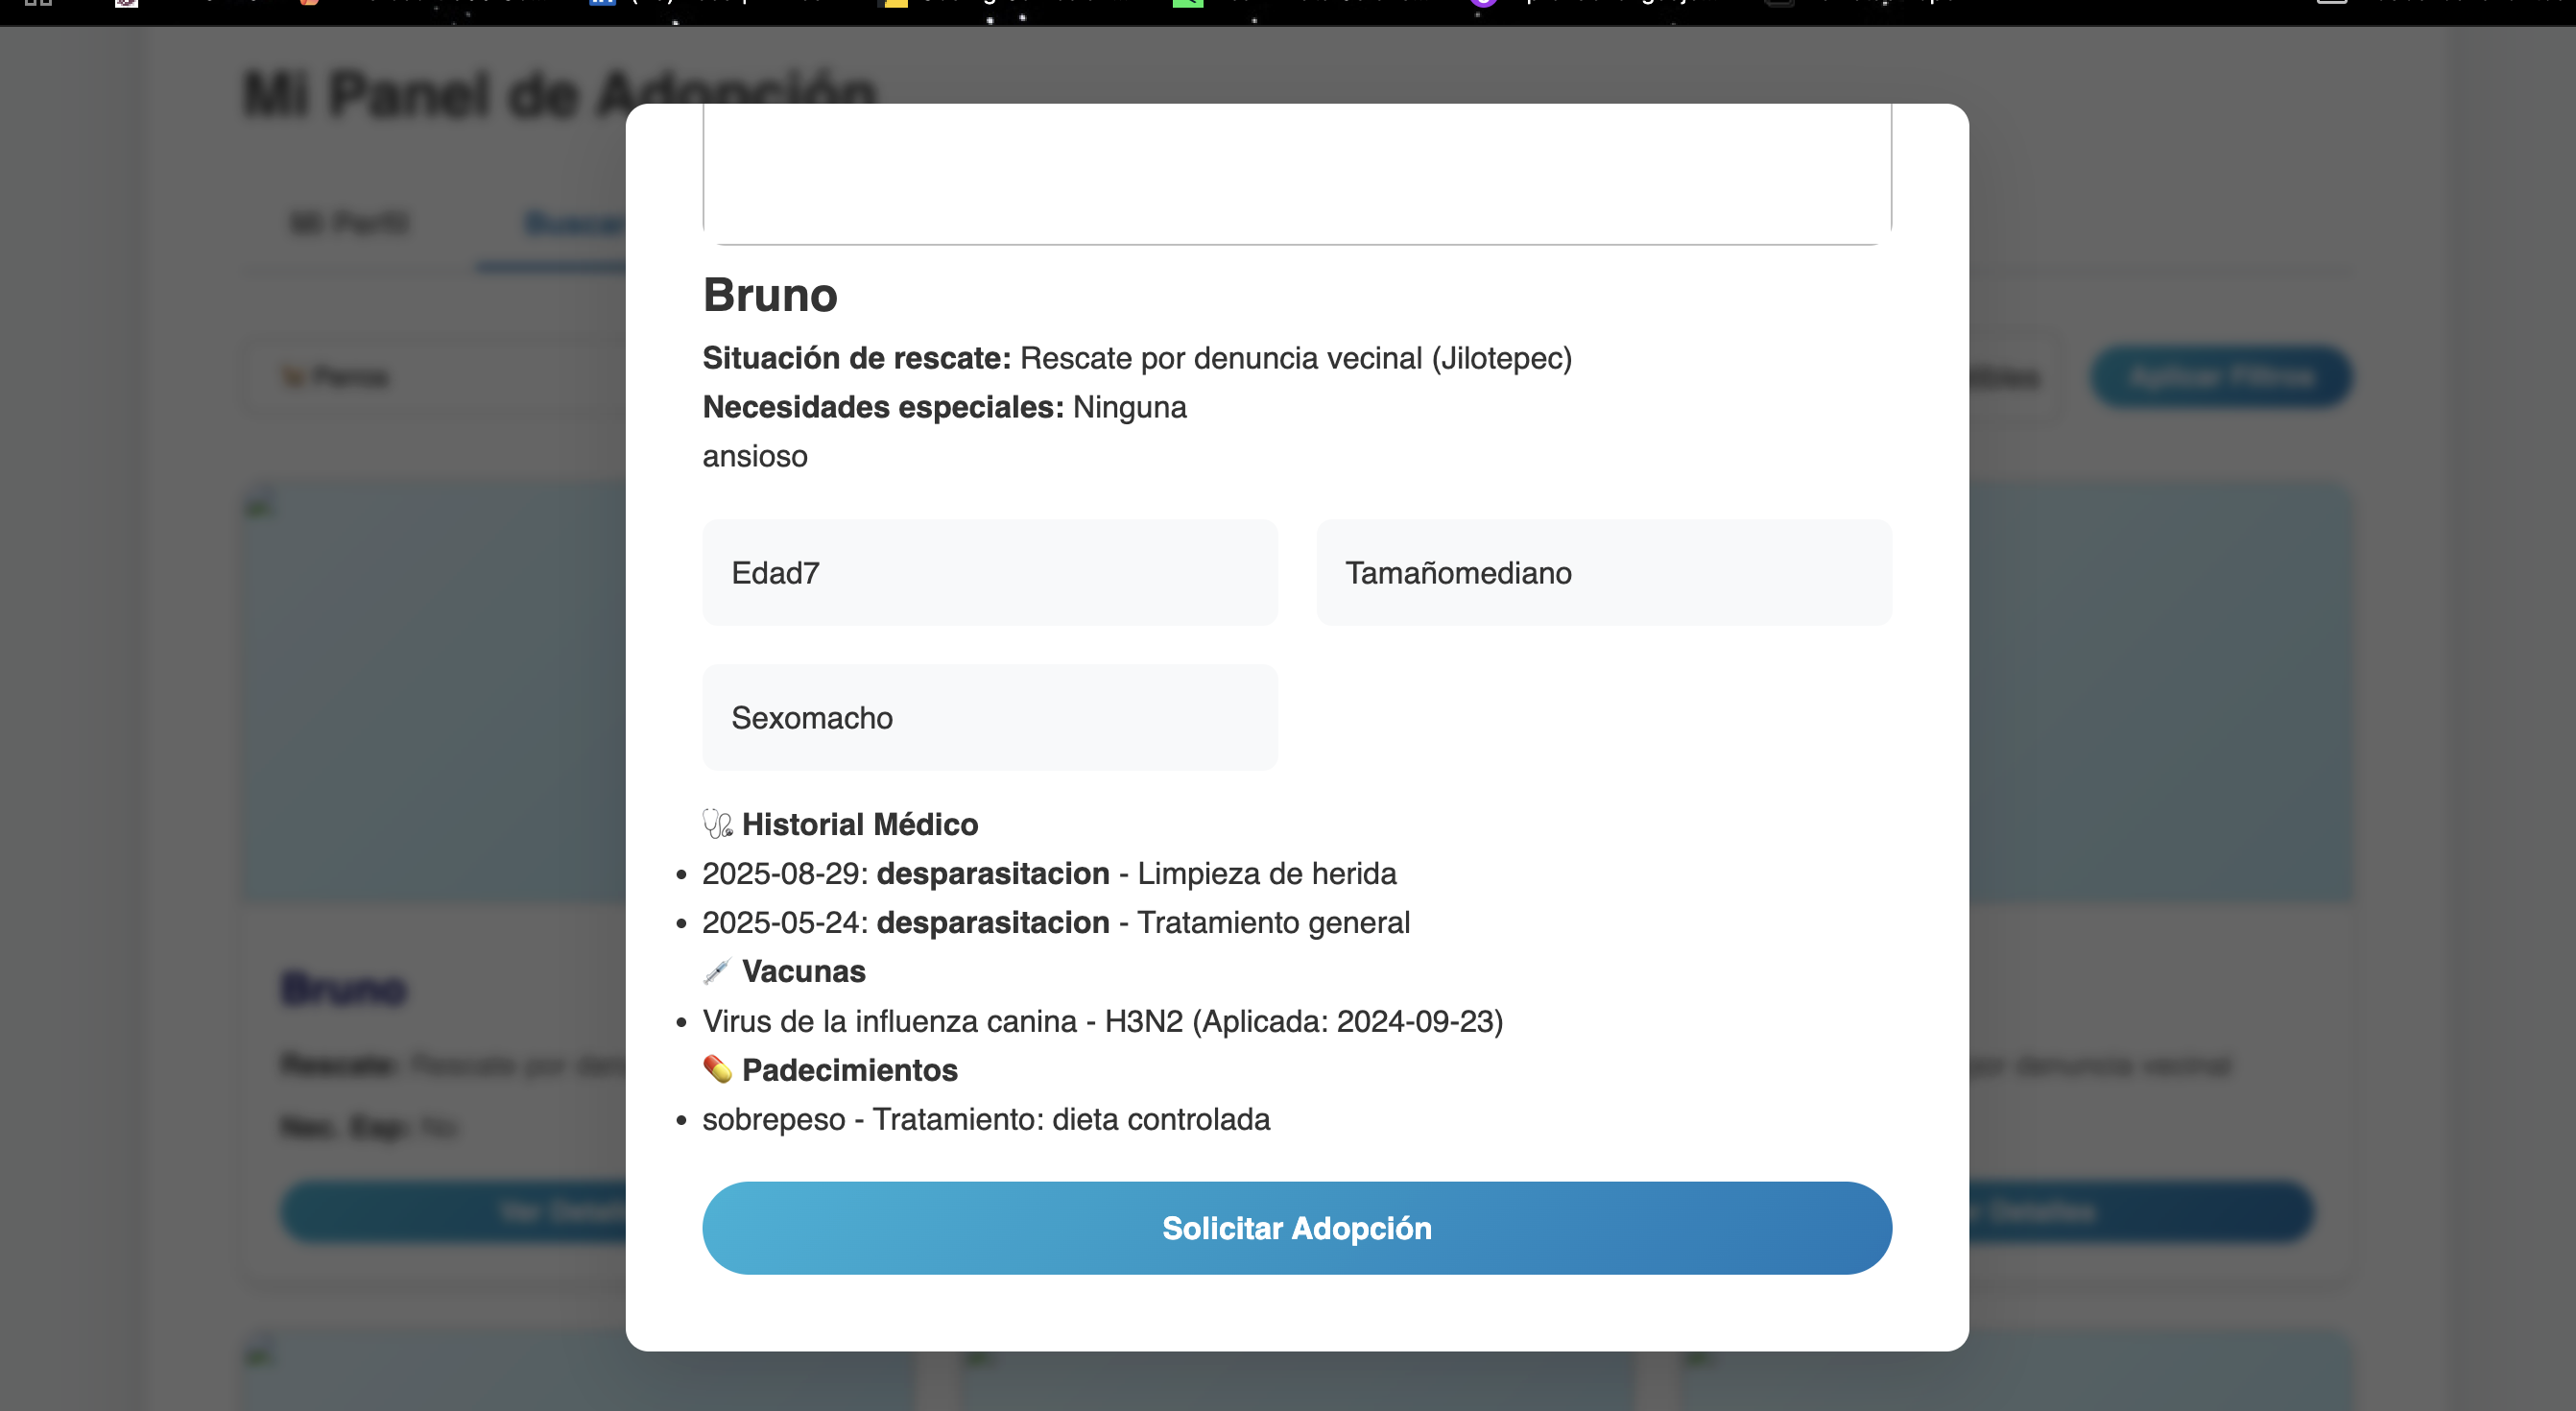
\includegraphics[width=0.8\textwidth]{Detalles mascotas.png} 
    \caption{Modal con Detalles Médicos y de Rescate}
    \label{fig:detalle}
\end{figure}

\subsubsection{3. Perfil de Idoneidad (Adoptante)}
Formulario exhaustivo validado que recopila información crítica para el algoritmo de emparejamiento:
\begin{itemize}
    \item Validación de dirección con API de Sepomex (CP dinámico).
    \item Cuestionario de vivienda (Tipo de inmueble, cercado, permiso de arrendador).
    \item Composición familiar y experiencia previa con mascotas.
\end{itemize}

\begin{figure}[H]
    \centering
    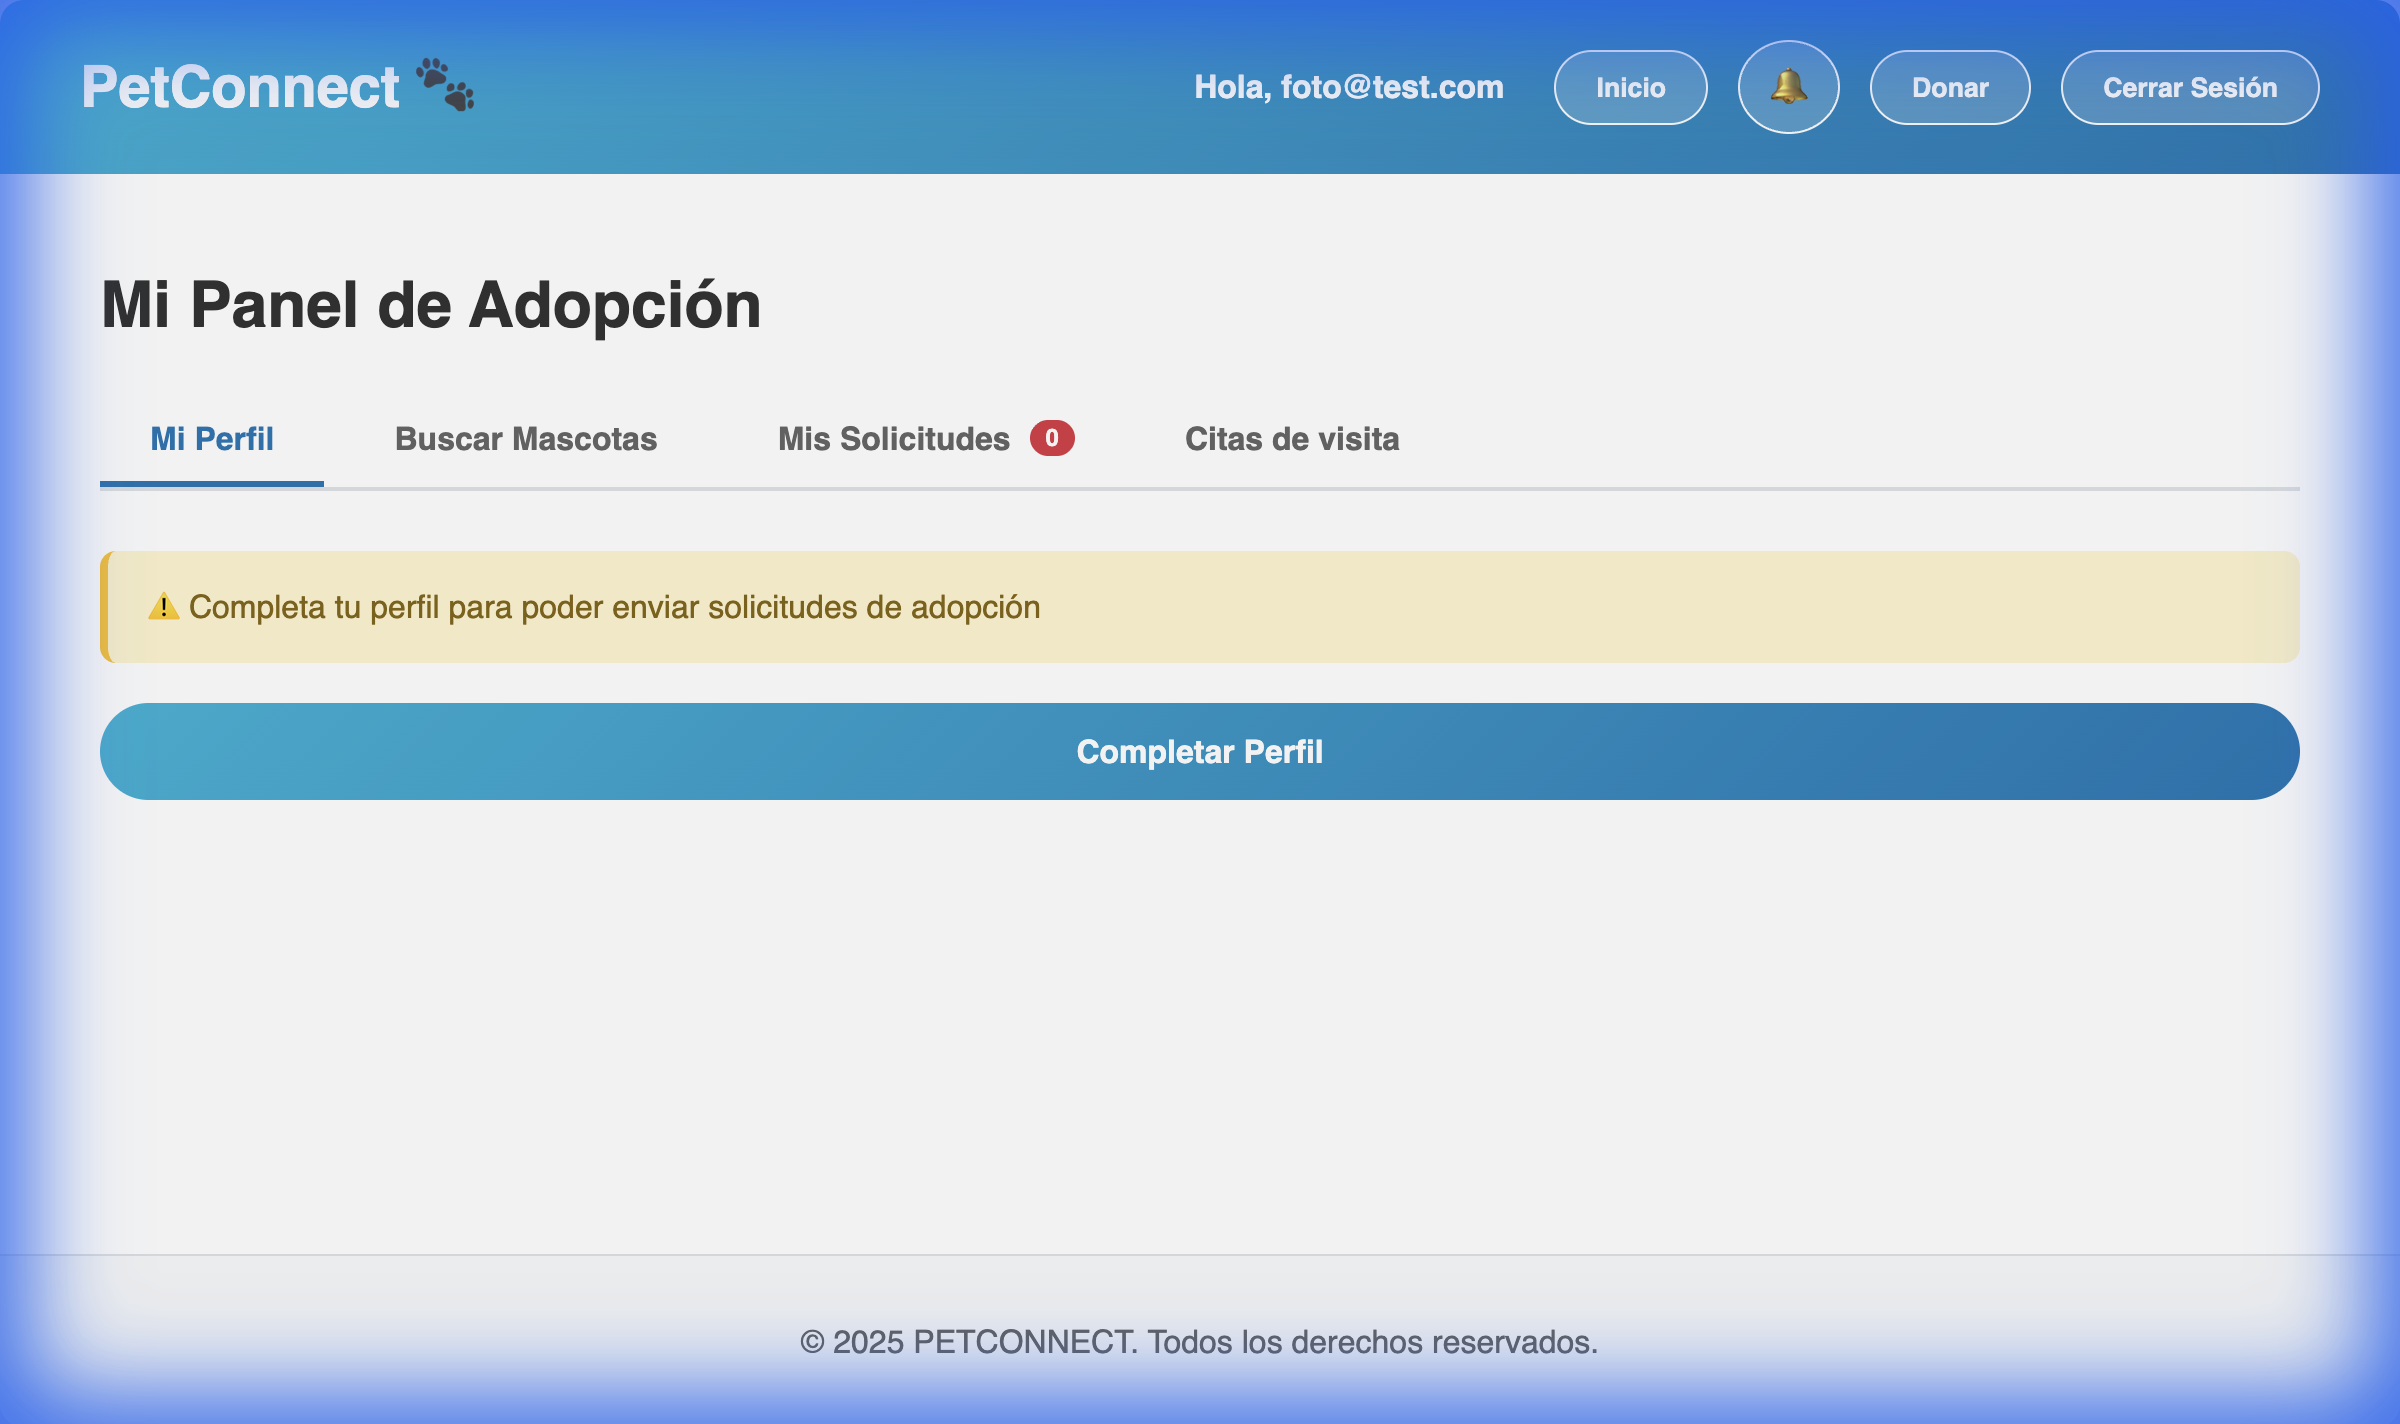
\includegraphics[width=0.8\textwidth]{Perfil_adoptante.png}
    \caption{Formulario de Perfil de Idoneidad}
    \label{fig:perfil}
\end{figure}

\subsubsection{4. Panel de Gestión (Fundación)}
Dashboard administrativo con pestañas para accesos rápidos:
\begin{itemize}
    \item \textbf{Alta de Rescates}: Formulario para registrar el evento origen de la mascota.
    \item \textbf{Control de Solicitudes}: Permite ver el perfil del solicitante y decidir la aprobación.
    \item \textbf{Alta de Colaboradores}: Módulo para registrar personal y asignar roles (ej. Cuidadores por turno).
    \item \textbf{Donaciones}: Visualización de donaciones recibidas.
    \item \textbf{Alta de Mascotas}: Formulario para registrar nuevas mascotas.
    \item \textbf{Lista negra}: Módulo para registrar dueños en lista negra por maltrato.
\end{itemize}

\begin{figure}[H]
    \centering
    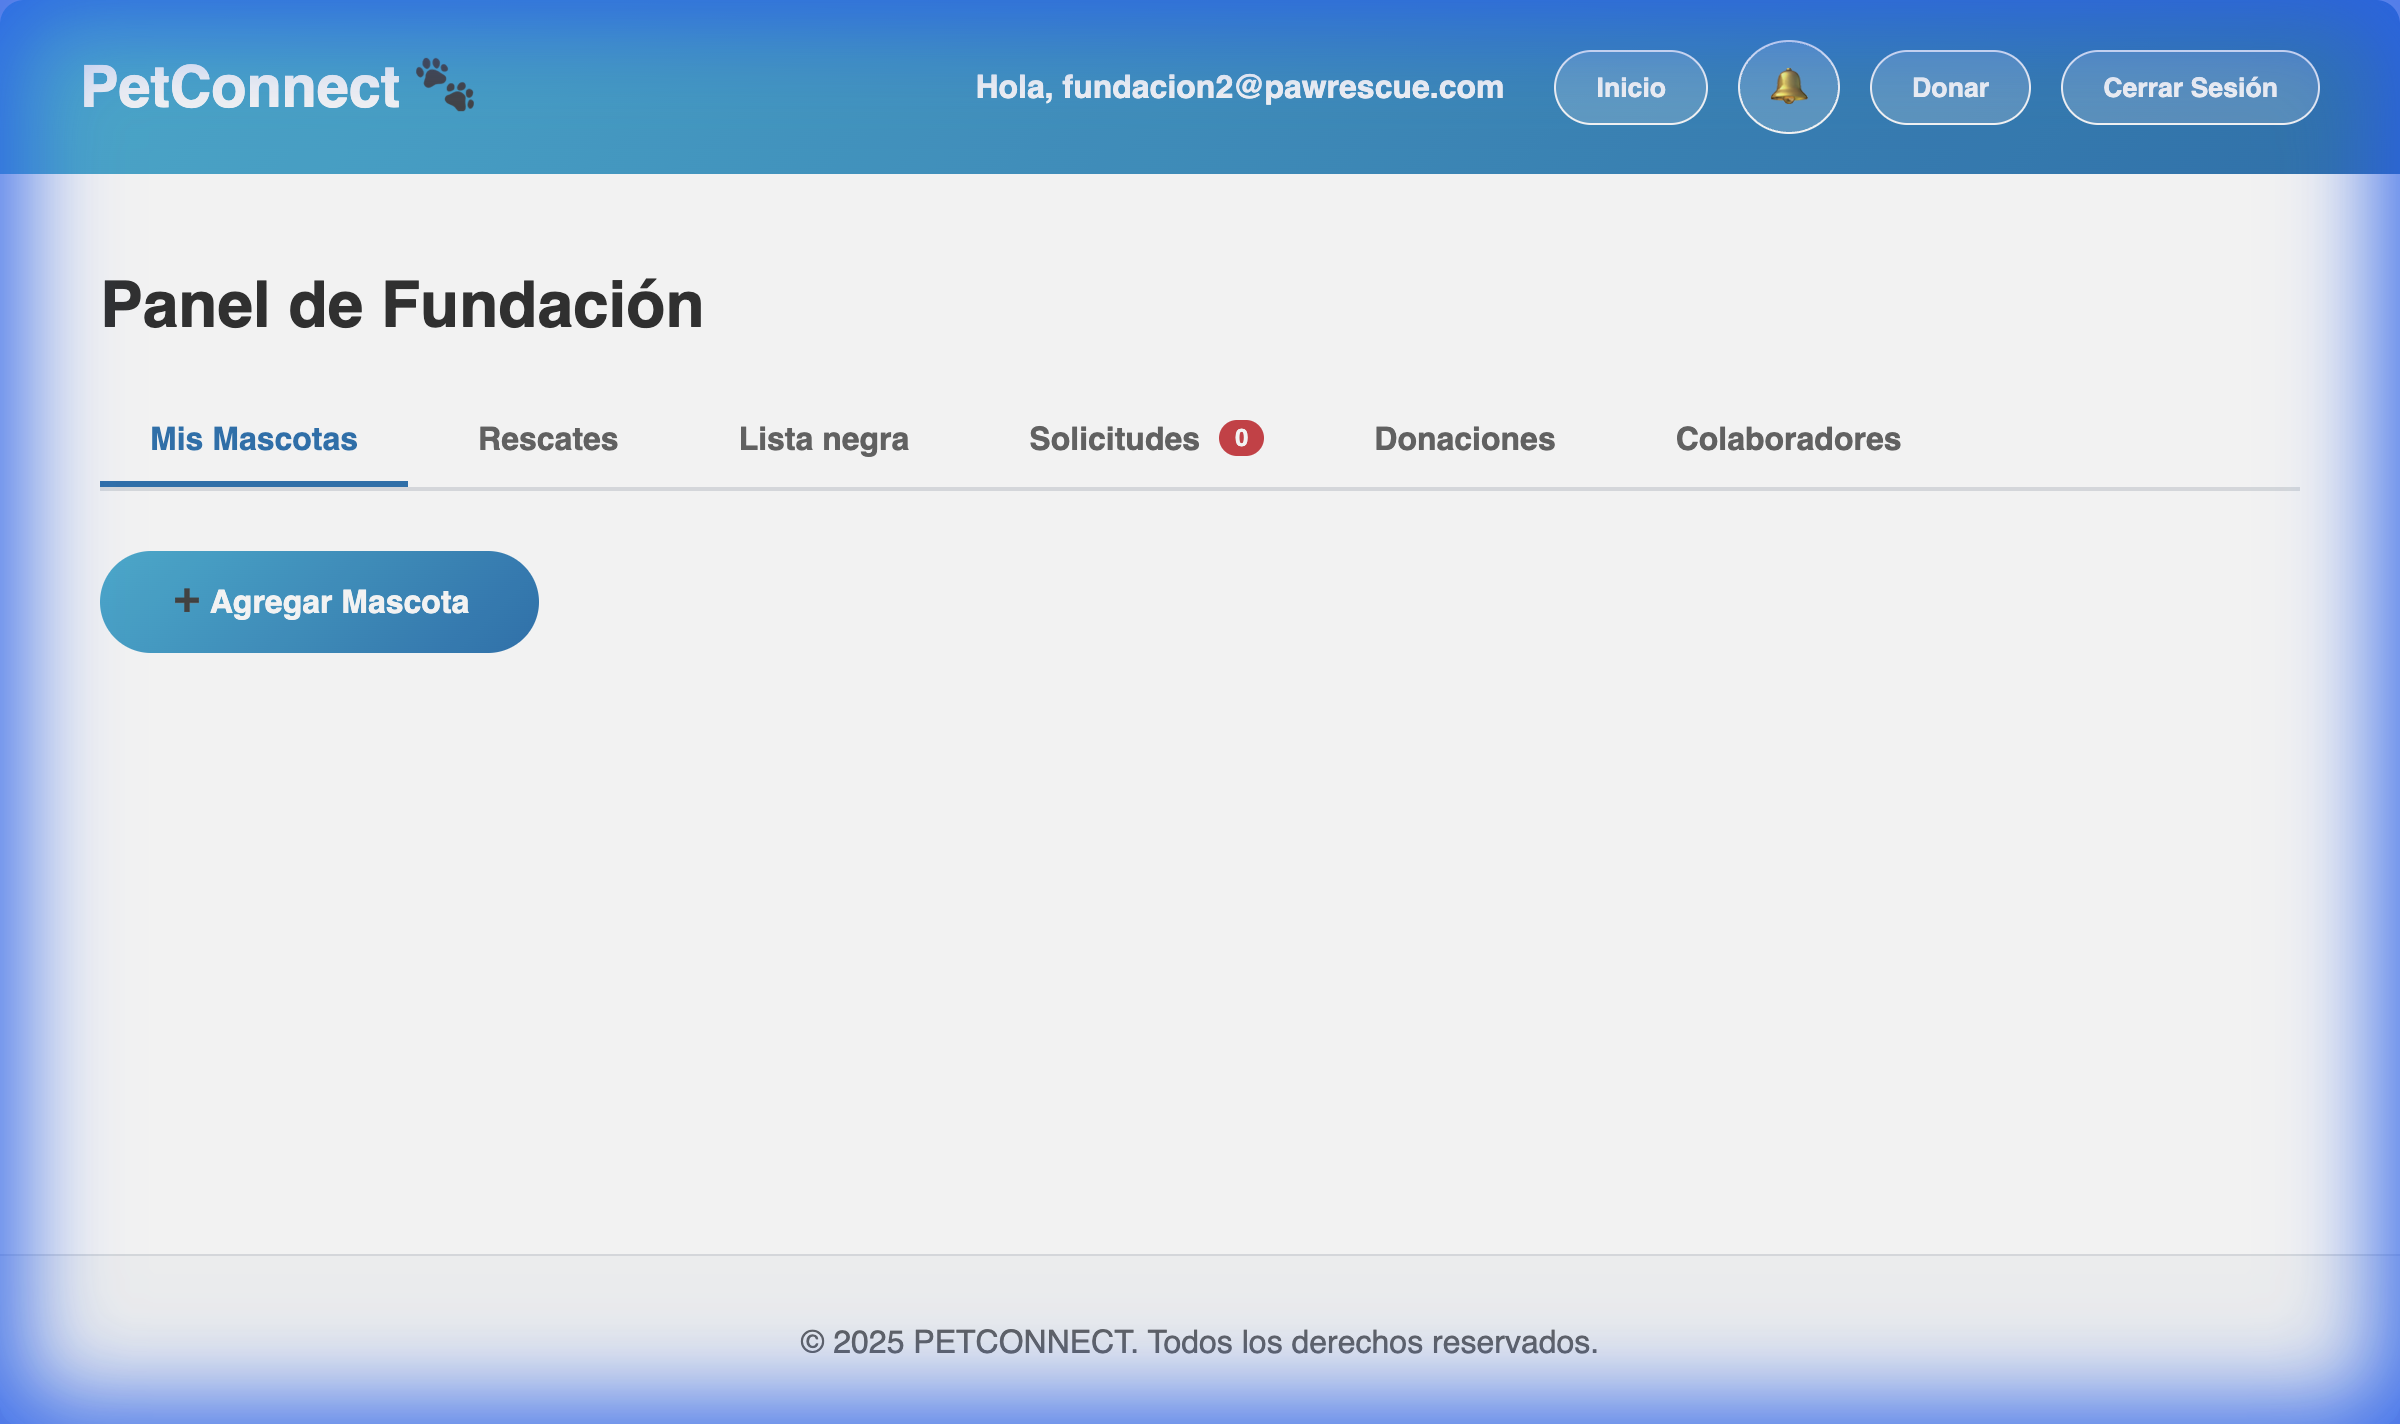
\includegraphics[width=0.8\textwidth]{Panel_fundacion.png}
    \caption{Dashboard de Administración para Fundaciones}
    \label{fig:fundacion}
\end{figure}

% 7. Diseño de Consultas
\newpage
\section{Consultas}

Consultas requeridas en Álgebra Relacional y SQL.

\subsection*{Consulta 1: Mascotas recuperadas HOY + datos rescate + personales}
Obtener el nombre, tamaño, sexo de las mascotas rescatadas en la fecha actual.

\textbf{Álgebra Relacional:}
\[
\pi_{nombre, tamanio, sexo, fecha, alcaldia} (\sigma_{fecha=HOY} (Mascota\_Rescatada \bowtie_{id\_mascota} Rescate))
\]

\textbf{SQL:}
\begin{lstlisting}
SELECT m.nombre, m.tamanio, m.sexo, r.fecha, r.alcaldia, r.situacion
FROM paw.mascota_rescatada m
JOIN paw.rescate r ON m.id_mascota = r.id_mascota
WHERE r.fecha = CURRENT_DATE;
\end{lstlisting}

\subsection*{Consulta 2: Mascotas recuperadas en "Gustavo A. Madero" en 2025}

\textbf{Álgebra Relacional:}
\[
\pi_{nombre, fecha} (\sigma_{alcaldia='Gustavo A. Madero' \land fecha \in [2025]} (Mascota\_Rescatada \bowtie Rescate))
\]

\textbf{SQL:}
\begin{lstlisting}
SELECT m.nombre, r.fecha, r.alcaldia
FROM paw.mascota_rescatada m
JOIN paw.rescate r ON m.id_mascota = r.id_mascota
WHERE r.alcaldia = 'Gustavo A. Madero' 
  AND r.fecha BETWEEN '2025-01-01' AND '2025-12-31';
\end{lstlisting}

\subsection*{Consulta 3: Personas a las que se les han quitado más de 1 mascota}

\textbf{Álgebra Relacional:}
\[
\pi_{nombre, num} (\sigma_{num > 1} (\gamma_{id\_duenio, nombre; count(id\_mascota)\to num} (Duenio \bowtie Mascota\_Duenio\_Hist)))
\]

\textbf{SQL:}
\begin{lstlisting}
SELECT d.nombre, COUNT(DISTINCT h.id_mascota) AS mascotas_retiradas
FROM paw.mascota_duenio_hist h
JOIN paw.duenio d ON d.id_duenio = h.id_duenio
GROUP BY d.id_duenio, d.nombre
HAVING COUNT(DISTINCT h.id_mascota) > 1
ORDER BY mascotas_retiradas DESC;
\end{lstlisting}

\subsection*{Consulta 4: Personas que han adoptado a más de 1 mascota}

\textbf{Álgebra Relacional:}
\[
\pi_{nombre, total} (\sigma_{total > 1} (\gamma_{id\_adoptante, nombre; count(id\_mascota)\to total} (Adoptante \bowtie Adopcion)))
\]

\textbf{SQL:}
\begin{lstlisting}
SELECT a.nombre AS nombre_adoptante, COUNT(ad.id_mascota) AS total_mascotas
FROM paw.adoptante a
JOIN paw.adopcion ad ON a.id_adoptante = ad.id_adoptante
GROUP BY a.id_adoptante, a.nombre
HAVING COUNT(ad.id_mascota) > 1;
\end{lstlisting}

\subsection*{Consulta 5: Relación Mascota-Adoptante idóneo}
Reglas para determinar idoneidad basadas en nivel económico, tipo de vivienda y características de la mascota.

\textbf{SQL:}
\begin{lstlisting}
SELECT adp.nombre AS adoptante, m.nombre AS mascota,
  CASE
    WHEN (p.nivel_economico = 'alto' AND r.necesidades_especiales IS NOT NULL) THEN 'Idoneo: Cuidados Especiales'
    WHEN (p.tipo_vivienda = 'casa-jardin' AND m.tamanio IN ('grande','mediano')) THEN 'Idoneo: Patio'
    WHEN (p.tipo_vivienda LIKE 'departamento%' AND m.tamanio = 'pequeño') THEN 'Idoneo: Departamento'
    ELSE 'No idoneo'
  END AS clasificacion
FROM paw.adoptante adp
JOIN paw.adoptante_perfil p ON p.id_adoptante = adp.id_adoptante
JOIN paw.mascota_rescatada m ON m.especie_id = 1
LEFT JOIN paw.rescate r ON r.id_mascota = m.id_mascota;
\end{lstlisting}

\subsection*{Consulta 6: Lista de visitantes que vendrán hoy (ordenadas por hora)}

\textbf{Álgebra Relacional:}
\[
\pi_{visitante, hora, mascota} (sort_{fecha\_hora} (\sigma_{fecha=HOY} (Cita\_Visita \bowtie Solicitud \bowtie Adoptante \bowtie Mascota)))
\]

\textbf{SQL:}
\begin{lstlisting}
SELECT a.nombre AS visitante, c.fecha_hora, m.nombre AS mascota
FROM paw.cita_visita c
JOIN paw.solicitud_adopcion s ON c.id_solicitud = s.id_solicitud
JOIN paw.adoptante a ON s.id_adoptante = a.id_adoptante
JOIN paw.mascota_rescatada m ON s.id_mascota = m.id_mascota
WHERE c.fecha_hora::date = CURRENT_DATE
ORDER BY c.fecha_hora ASC;
\end{lstlisting}

\subsection*{Consulta 7: Perros adoptados este mes en la CDMX}

\textbf{Álgebra Relacional:}
\[
\pi_{mascota, fecha, estado} (\sigma_{mes=actual \land estado=CDMX} (Adopcion \bowtie Mascota \bowtie AdoptantePerfil \bowtie Sepomex))
\]

\textbf{SQL:}
\begin{lstlisting}
SELECT m.nombre, a.fecha_adopcion, 'CDMX' as estado
FROM paw.adopcion a
JOIN paw.mascota_rescatada m ON m.id_mascota = a.id_mascota
JOIN paw.adoptante_perfil p ON p.id_adoptante = a.id_adoptante
JOIN sepomex.codigos c ON c.codigo_postal = p.codigo_postal
WHERE m.especie_id = 1
  AND a.fecha_adopcion >= date_trunc('month', CURRENT_DATE)
  AND c.entidad_id = 9; -- CDMX
\end{lstlisting}

\subsection*{Consulta 8: Cuidadores que han venido todos los días de la semana}

\textbf{SQL:}
\begin{lstlisting}
WITH dias_semana AS (
   SELECT generate_series(CURRENT_DATE - 6, CURRENT_DATE, '1 day')::date AS dia
)
SELECT e.nombre, COUNT(DISTINCT a.fecha) as dias_asistidos
FROM paw.cuidadores c
JOIN paw.empleados e ON e.id_empleado = c.id_empleado
JOIN dias_semana d ON TRUE
LEFT JOIN paw.asistencia a ON a.id_empleado = c.id_empleado AND a.fecha = d.dia
GROUP BY e.id_empleado, e.nombre
HAVING COUNT(DISTINCT a.fecha) = 7;
\end{lstlisting}

\subsection*{Consulta 9: Empleados que han laborado en todas las sucursales}
División Relacional.

\textbf{Álgebra Relacional:}
\[
Empleados\_Todas\_Sucursales \leftarrow \pi_{id\_empleado, id\_sucursal}(Empleado\_Sucursal\_Hist) \div \pi_{id\_sucursal}(Sucursal)
\]

\textbf{SQL:}
\begin{lstlisting}
SELECT e.nombre
FROM paw.empleados e
JOIN paw.empleado_sucursal_hist h ON h.id_empleado = e.id_empleado
GROUP BY e.id_empleado, e.nombre
HAVING COUNT(DISTINCT h.id_sucursal) = (SELECT COUNT(*) FROM paw.sucursal);
\end{lstlisting}

\subsection*{Consulta 10: Perros que tienen todas sus vacunas al corriente}

\textbf{SQL:}
\begin{lstlisting}
SELECT m.nombre
FROM paw.mascota_rescatada m
WHERE m.especie_id = 1
  AND NOT EXISTS (
    SELECT 1 FROM paw.vacuna_aplicada va
    WHERE va.id_mascota = m.id_mascota
      AND va.proxima_dosis < CURRENT_DATE
  );
\end{lstlisting}

\end{document}